%% LyX 2.1.4 created this file.  For more info, see http://www.lyx.org/.
%% Do not edit unless you really know what you are doing.
\documentclass[spanish]{scrartcl}
\usepackage[T1]{fontenc}
\usepackage[latin9]{inputenc}
\usepackage{array}
\usepackage{multirow}
\usepackage{amsmath}
\usepackage{amssymb}

\makeatletter

%%%%%%%%%%%%%%%%%%%%%%%%%%%%%% LyX specific LaTeX commands.
%% Because html converters don't know tabularnewline
\providecommand{\tabularnewline}{\\}

%%%%%%%%%%%%%%%%%%%%%%%%%%%%%% User specified LaTeX commands.
\usepackage{tikz}

\makeatother

\usepackage{babel}
\addto\shorthandsspanish{\spanishdeactivate{~<>}}

\begin{document}
Apuntes de clase Mi�rcoles 13/03/2019


\section*{M�dulo}

Definici�n del valor absoluto de un numero real

\[
\mid{-7}\mid=7
\]


\[
\mid{3}\mid=3
\]


\[
\mid{a}\mid=\begin{cases}
\begin{array}{c}
a\\
-a
\end{array} & \begin{array}{c}
si\,a>0\\
si\,a<0
\end{array}\end{cases}
\]
Propiedades del valor absoluto

Propiedad 1

\begin{equation}
\begin{array}{cc}
\mid{a}\mid=k & con\,k>0\iff a=\pm k\end{array}
\end{equation}


Ej. 1

\[
\begin{array}{cc}
\mid{a}\mid=2 & ecuaci\acute{o}n\end{array}
\]


\begin{eqnarray*}
Si\,a\ge0 & \vee & Si\,a<0\\
\mid{a}\mid=2 &  & \mid{a}\mid=2\\
a=2 &  & -a=2\\
 &  & a=-2
\end{eqnarray*}


Ej. 2

\begin{eqnarray*}
Si\,2x+3\ge0 & \vee & Si\,2x+3<0\\
x\ge\frac{-3}{2} &  & x<\frac{-3}{2}\\
\left[\frac{-3}{2};+\infty\right) &  & \left(-\infty;\frac{-3}{2}\right]\\
\mid{2x+3}\mid=7 &  & \mid{2x+3}\mid=7\\
2x+3=7 &  & -({2x+3})=7\\
2x=7-3 &  & -2x-3=7\\
x=\frac{4}{2} &  & -2x=10\\
\boxed{x=2} &  & x=\frac{-10}{2}\\
\in\left[\frac{-3}{2};+\infty\right) &  & \boxed{x=-5}\\
 &  & \in\left(+\infty;\frac{-3}{2}\right]\\
 & \boxed{S=S_{1}\cup S_{2}=\{2;-5\}}
\end{eqnarray*}


Ej. 3

\[
\begin{array}{c}
\mid{x}\mid=k\end{array}\begin{array}{c}
con\end{array}k>0
\]


\begin{eqnarray*}
si\,x\ge0 & \vee & si\,x<0\\
\mid{x}\mid=k &  & \mid{x}\mid=k\\
x=k &  & -x=k\\
 &  & x=-k\\
 & S=S_{1}\cup S_{2}=\{+k;-k\}\\
 & \boxed{x=\pm k}
\end{eqnarray*}


Usando la propiedad

\begin{eqnarray*}
 & \mid{3x-2}\mid=4\\
 & \boxed{3x-2=\pm4}\\
3x-2=4 &  & 3x-2=-4\\
3x=4+2 &  & 3x=-4+2\\
x=\frac{6}{3} &  & 3x=-2\\
x=2 &  & x=\frac{-2}{3}
\end{eqnarray*}


Propiedad 2

\begin{equation}
\begin{array}{cc}
\mid{x}\mid<k & con\,k>0\Rightarrow-k<x<k\end{array}
\end{equation}


Ej. 1

\begin{eqnarray*}
 & \mid{x}\mid<6\\
Si\,x\ge0 &  & Si\,x<0\\
\mid{x}\mid<6 &  & \mid{x}\mid<6\\
x<6 &  & -x<6\\
\boxed{S_{1}=[0;6)} &  & x>-6\\
 &  & \boxed{S_{2}=(-6;0)}
\end{eqnarray*}


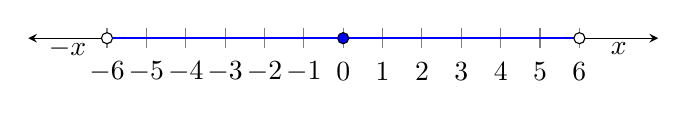
\begin{tikzpicture}[x=5mm,y=1.2em]
\draw[stealth-stealth] (-8,0) -- (8,0);
\foreach \x [count=\xi] in {-6,...,6}
{\node at (\x,-1) {$\x$};
\draw[gray] (\x,0.3) -- (\x,-0.3);}
\draw[blue,thick] (-6,0) -- (6,0);
\fill[blue,draw=black,thin] (0,0) circle (2pt);
\fill[white,draw=black,thin] (-6,0) circle (2pt);
\fill[white,draw=black,thin] (6,0) circle (2pt);
\node at (7, -0.3) {$x$};
\node at (-7, -0.3) {$-x$};
\end{tikzpicture}

\[
-6<x<6
\]



\section*{Entorno}

Se llama Entorno de centro $a$ y radio $r$ y se escribe $E(a;r)$
al conjunto de n�meros reales que verifican:

\[
\begin{array}{cc}
E(a;r)=\left\{ x\in\mathbb{R}/\mid{x-a}\mid<r\right\}  & con\,a=centro;r=radio\end{array}
\]


Ej.

\[
E(7,3)
\]


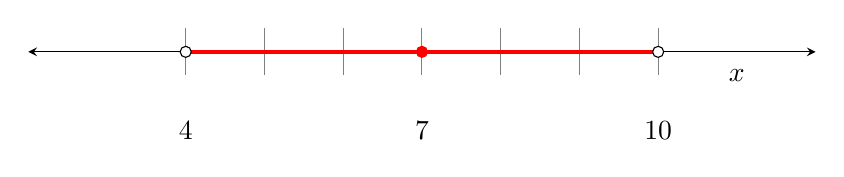
\begin{tikzpicture}
\draw[stealth-stealth] (2,0) -- (12,0);
\foreach \x [count=\xi] in {4,...,10}{
\draw[gray] (\x,0.3) -- (\x,-0.3);}
\node at (4, -1) {4};
\node at (7, -1) {7};
\node at (10, -1) {10};
\node at (11, -0.3) {$x$};
\draw[red,very thick] (4,0) -- (10,0);
\fill[white,draw=black,thin] (4,0) circle (2pt);
\fill[white,draw=black,thin] (10,0) circle (2pt);
\fill[red,draw=red,thin] (7,0) circle (2pt);
\end{tikzpicture}

\[
\begin{array}{c}
E(7;3)=(4;10)\\
E(7;3)=\{x\in\mathbb{R}/\mid{x-7}\mid<3\}\\
\mid{x-7}\mid<3\\
\boxed{-3<x-7<3}\\
-3+7<x<3+7\\
\boxed{{4<x<10}}\\
(4;10)
\end{array}
\]



\section*{Entorno Reducido}

Se llama Entorno Reducido de centro $a$ y radio $r$ y se escribe
$E^{*}(a;r)$ al conjunto de n�meros reales que verifican:

\[
E^{*}(a;r)=\{x\in\mathbb{R}/0<\mid{x-a}\mid<r\}
\]


Ej.

\[
\begin{array}{c}
E^{*}(0;2)=\{x\in\mathbb{R}/0<\mid{x-0}\mid<2\}\\
(-2;0)\cup(0;2)
\end{array}
\]


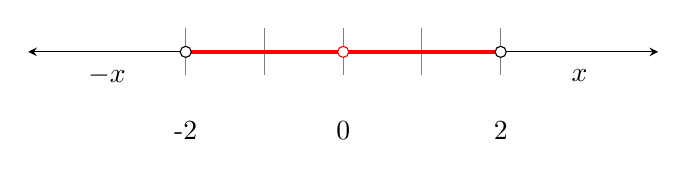
\begin{tikzpicture}
\draw[stealth-stealth] (-4,0) -- (4,0);
\foreach \x [count=\xi] in {-2,...,2}{
\draw[gray] (\x,0.3) -- (\x,-0.3);}
\node at (-2, -1) {-2};
\node at (0, -1) {0};
\node at (2, -1) {2};
\node at (3, -0.3) {$x$};
\node at (-3, -0.3) {$-x$};
\draw[red,very thick] (-2,0) -- (2,0);
\fill[white,draw=black,thin] (-2,0) circle (2pt);
\fill[white,draw=black,thin] (2,0) circle (2pt);
\fill[white,draw=red,thin] (0,0) circle (2pt);
\end{tikzpicture}


\section*{Concepto de L�mite}

\[
f(x)=x+3
\]


\[
\lim_{x\to4}f(x)\Rightarrow\lim_{x\to4}(x+3)
\]


\[
x\,tiende\,a,\,x\,se\,acerca\,a
\]


\begin{tabular}{|c|c|c|}
\hline 
$x$ & $f(x)$ & \tabularnewline
\hline 
\hline 
3.99 & 6.99 & \multirow{3}{*}{$L_{1}=\lim\limits _{x\to4^{-}}(x+3)=7$}\tabularnewline
\cline{1-2} 
3.999 & 6.999 & \tabularnewline
\cline{1-2} 
3.9999 & 6.9999 & \tabularnewline
\hline 
4 & 7 & \tabularnewline
\hline 
4.0001 & 7.0001 & \multirow{3}{*}{$L_{2}=\lim\limits _{x\to4^{+}}(x+3)=7$}\tabularnewline
\cline{1-2} 
4.001 & 7.001 & \tabularnewline
\cline{1-2} 
4.01 & 7.01 & \tabularnewline
\hline 
\end{tabular}

Existen l�mites laterales y son iguales.

\[
L_{1}=L_{2}\Rightarrow\exists\lim_{x\to4}(x+3)=7
\]

\end{document}
